% !TeX spellcheck = en_GB
\section{Background Theory}
We derive here a mathematical basis on fractals and dimensions of sets.
This will be used later in our more specific study of random fractals.

\subsection{Dimensions}
The concept of dimension is quite intuitive from an everyday life perspective.
However, the mathematical concept is more involved.
From the non-mathematical world, this can be used to have better understanding of other object arising from other fields such as DNA structure\footnote{\url{https://news.mit.edu/2009/3d-genome}}, or lungs\cite{IOLMSD_2009}.

\subsubsection{Intuition}
Some objects that we are used to working with have an established dimension:
\begin{itemize}
	\item \textbf{Empty set} / \textbf{Point}: dimension 0
	\item \textbf{Curve} (e.g.: \textit{line}): dimension 1
	\item \textbf{Surface} (e.g.: \textit{square}): dimension 2
	\item \textbf{Volume} (e.g.: \textit{cube}): dimension 3
	%\item \textbf{General $d$-dim set} (e.g.: \textit{$d$-dimensional cuboid}): dimension $d$
\end{itemize}
All of these usual objects have integral dimensions, making it (relatively) easy to understand.

A rule of thumb to calculate the dimension is to double (or, in general, multiply by $n$) the size of the object, and count the number of copies of the original object obtained.
If there are $N$ original objects, the dimension is $d = \frac{\ln(N)}{\ln(n)}$.
This is so that when scaling by $n$, the length/area/volume of the set is multiplied by $N = n^d$.

Some objects have a more complicated dimension (in fact, a non-integral one)\footnote{This will be discussed in more detail in \ref{fractalsExamples}.}:
\begin{itemize}
	\item \textbf{Cantor Set} (see fig. \ref{fig:CantorSet}): dimension $\log_3(2) = \frac{\ln(2)}{\ln(3)} \simeq 0.631$
	\item \textbf{Koch Snowflake} (see fig. \ref{fig:KochSnowflake}): dimension $\log_3(4) = \frac{\ln(4)}{\ln(3)} \simeq 1.262$
	\item \textbf{Sierpiński Carpet} (see fig. \ref{fig:SierpinskiCarpet}): dimension $\log_2(8) = \frac{\ln(8)}{\ln(3)} \simeq 1.893$
\end{itemize}
The fractional dimensions of these objects justify creating a formal mathematical definition.

After this quick overview, 3 properties seem desirable for a definition of dimension \cite{Pollicott_LFDT}.
For a set $X$ ($\subset \R^n$, in general):
\begin{enumerate}\label{propr:desirable}
	\item If $X$ is a manifold, then the dimension should coincide with our natural preconception. \label{propr:desirable1}
	\item In some cases, $X$ may have a fractional (i.e. non-integral) dimension. \label{propr:desirable2}.\\
	This is needed in order to describe sets as the ones discussed above.
	\item If $X$ is countable, then $X$ has dimension $0$. \label{propr:desirable3}
\end{enumerate}
There are several definition for dimension, satisfying different properties.

\subsubsection{Topological Dimension}
The topological dimension is the most straightforward way to define dimension.
It relies on the intuition that the boundary of a ball of dimension $d$ should have dimension $d-1$.

\begin{definition}[Topological dimension]\label{def:topologicalDimension}
	The topological dimension $\dim_T(X)$ of a set $X$ is defined recursively through the following:
	\begin{equation*}
		\dim_T(X) =
		\begin{cases}
			-1 & \text{if } \ X = \emptyset \\
			 d & \text{if } \ d = \min \left\lbrace n \in \N \mid \forall x \in X, \ \exists \, r>0 \text{ s.t. } \dim_T(\partial B_r(x) \cap X) \leq n-1 \right\rbrace
		\end{cases}
	\end{equation*}
\end{definition}

This definition satisfies the first desired property (\ref{propr:desirable}:\ref{propr:desirable1}).
However, $\dim_T$ is always an integer (this is clear from definition).
Therefore, it does not satisfy the second desired property (\ref{propr:desirable}:\ref{propr:desirable2}).

\subsubsection{Box Dimension}
The box dimension is more general than the topological one, in the sense that it allows non-integral dimensions.
It relies on an intuition mentioned before: when scaled by $n$, a set contains $N$ copies of the original set, then the dimension should be  $\frac{\ln(N)}{\ln(n)}$.

\begin{definition}[Box dimension]\label{def:boxDimension}
	The box dimension $\dim_B$ of a set $X$ is defined through the following limit:
	$$
	\dim_B(X) = \lim_{\varepsilon \to 0} \frac{\ln(N(\varepsilon))}{-\log(\varepsilon)}
	$$
	Here, $N(\varepsilon)$ is the smallest number of $\varepsilon$-balls needed to cover $X$.
	
	Note that box dimension exists only if this limit exists.
	In the case this limit does not exist, it is possible to define upper and lower box dimensions, taking respectively $\limsup$ and $\liminf$ in the definition above.
	(Both upper and lower box dimension with the general box dimension when it exists.) 
\end{definition}

This definition satisfies the first and second desired property (\ref{propr:desirable}:\ref{propr:desirable1},\ref{propr:desirable2}).
However, if we consider $X = \{0\} \cup \{\frac{1}{n} \mid n \in \N^*\}$, then $\dim_B(X) > 0$, but $X$ is countable.
Therefore, it does not satisfies the third desired property (\ref{propr:desirable}:\ref{propr:desirable3}).

\subsubsection{Hausdorff Dimension}
The Hausdorff dimension (sometimes also called fractal dimension) is considered to be the most robust concept of dimension.
The reason of this consortium is that Hausdorff dimension has a measure (the Hausdorff measure) associated to it).
The definition is more involved than both the topological and the box dimensions.

\begin{definition}[Hausdorff/fractal dimension]\label{def:HausdorffDimension}
	The Hausdorff dimension $\dim_H$ of a set $X$ is defined as follows:
	$$\text{For } \varepsilon > 0, \ d \geq 0, \quad
	H_{\varepsilon}^d(X) = 
	\inf_{\substack{\mathcal{U} \text{ open cover of } X\\
			U \in \, \mathcal{U} \implies \diam{U} < \varepsilon}}
		\left\lbrace \sum_{U \in \, \mathcal{U}} \diam{U}^d \right\rbrace
	$$
	A $H_{\varepsilon}^d(X)$ is an increasing function as $\varepsilon \to 0$, the following limit is well defined:
	$$
	H^d(X) = \lim_{\varepsilon \to 0} H_{\varepsilon}^d(X)
	$$
	This defines a measure, which is called the $d$-dimensional Hausdorff measure.
	
	For a set $X$, $H^d(X)$ jumps from $0$ to $\infty$, when $d$ varies from $0$ to $\infty$ (this will be proved as a claim, see\ref{propr:Hausdorff_jump}).
	The particular value at which this jump occurs is the Hausdorff dimension of $X$. Formally:
	$$
	\dim_H(X) = \inf \{ \delta \mid H^{\delta}(X) = 0 \}
	$$
\end{definition}

This definition satisfies all three of the desired property (\ref{propr:desirable}:\ref{propr:desirable1},\ref{propr:desirable2},\ref{propr:desirable3}).
The first two are clear from definition.
\begin{property}
	Countable sets have Hausdorff dimension 0.
\end{property}
\begin{proof}
	Suppose $X = \{ x_n \mid n \in \N \}$ is countable.
	Let $\varepsilon > 0$, and take $\{ \varepsilon_n \mid n \in \N \}$ such that $\sum_{n=0}^{\infty} \varepsilon_n^d < \varepsilon$.
	Then $\mathcal{B} = \{ B(x_n,\varepsilon_n) \mid n \in \N \}$ is an open cover of $X$, so $H_{\varepsilon}^d(X) \leq \varepsilon$.
	As this is true $\forall \varepsilon > 0, \ \forall d \geq 0$, get $H^d(X) = 0$ for all $d \geq 0$.
	So finally, $\dim_H(X) = 0$.
\end{proof}

The Hausdorff dimension is usually harder to calculate in practice.

\subsubsection{Some Relations Between Dimensions}
For dimension definition, there is a choice to make between more robust, but hard to calculate (Hausdorff dimension) and less robust but easier to calculate (Topological/Box dimension) definitions.
It is therefore very useful to know some relationships between the three notions (it is then possible to use, for example, box dimension to give estimates for the Hausdorff dimension).

\begin{property}[Upper bound for fractal dimension]
	Box dimension is greater than or equal to Hausdorff dimension.
\end{property}
\begin{proof}
	For a set $X$ (with box dimension well defined):
	Let $\eta > 0$, $\gamma = \dim_B(X) + \eta$ and $\delta = \dim_B(X) + 2\eta$.
	Then, $\exists \, \varepsilon > 0$ such that $X$ can be covered by $N(\varepsilon) < \varepsilon^{-\gamma}$ $\varepsilon$-balls.
	Thus, $H_{\varepsilon}^{\delta}(X) \leq \varepsilon^{-\gamma}\varepsilon^{\delta} = \varepsilon^{\eta}$, so $H^{\delta}(X) = 0$.
	This gives $\dim_H(X) < \dim_B(X) + 2\eta \quad \forall \eta > 0$, and hence, $\dim_H(X) \leq \dim_B(X)$.
\end{proof}

Thus, by calculating the box dimension, we also have an upper bound for the Hausdorff dimension.

\begin{lemma}
	If the $d$-dimensional Lebesgue measure is non-zero, then the Hausdorff dimension is greater than or equal to d.
\end{lemma}
\begin{proof}
	Suppose a set $X$ is such that $\dim_H(X)<d$.
	\begin{claim}\label{propr:Hausdorff_jump}
		$H^d(X) < \infty \implies H^c(X) = 0 \quad \forall c > d$
	\end{claim}
	\begin{proof}
		As $H^d(X) < \infty$: For all $\varepsilon > 0$ there is an open cover $\mathcal{U}$ for $X$ such that $\sum_{U \in \mathcal{U}} \diam{U}^d < \infty$ and $\diam{U} < \varepsilon$.
		So
		$$\sum_{U \in \, \mathcal{U}} \diam{U}^c \leq
		\underbrace{\varepsilon^{c-d}}_{\substack{\to 0\\\text{as } \varepsilon \to 0}} \ 
		\underbrace{\sum_{U \in \, \mathcal{U}} \diam{U}^d}_{< \infty}
		\to 0 \quad \text{ as } \varepsilon \to 0
		$$
	\end{proof}
	Thus, $H^d(X) = 0$.
	Now, the $d$-dimensional Hausdorff measure is a rescaling of the usual $d$-dimensional Lebesgue measure, so $\Lambda_d(X) = 0$ \footnote{Writing $\Lambda_d(X)$ for the $d$-dimensional Lebesgue measure of $X$.}.
	This completes the proof by taking the contrapositive.
\end{proof}

Thus, finding a $d$ such that the Lebesgue measure is non-zero gives a lower bound for the Hausdorff dimension.

\begin{property}[Lower bound for fractal dimension]
	Topological dimension is less than or equal to Hausdorff dimension.
\end{property}
\begin{proof}
	This follows directly from the last property, as a set $X$ having Topological dimension $d$ (i.e. $\dim_T(X) = d$) implies that its $d$-dimensional Lebesgue measure will be positive (i.e. $\Lambda_d(X) > 0$).
\end{proof}

In fact, the Hausdorff dimension is bounded by the topological dimension and the box dimension, i.e. for any set $X$, $\dim_T(X) \leq \dim_H(X) \leq \dim_B(X)$.

%%%%%%%%%%%%%%%%%%%%%%%%%%%%%%%%%%%%%%%%%%%%%%%%%%%%%%%%%%%%%%%%%%%%%%%%%%%%%%%%
\subsection{Fractals}
The first traces of fractals come back to the 17th century with the mathematician and philosopher Gottfried Leibniz, philosophizing about recursive self-similarity.
Proper sketches of a mathematical definition for fractals only go back to Karl Weierstrass, during the 19th century.
The recursive self-similarity pattern of most common fractals made their fame:
images of some fractals (e.g. Julia sets, Koch snowflake, Sierpiński gasket) have become popular across the mathematics and non-mathematics world.

\subsubsection{Formal Definition}
There is a controversial mathematical definition of fractals (introduced by Benoît Mandelbrot):
\begin{definition}[Fractal]\label{def:fractal}
	A fractal is a subset of Euclidean space with a Hausdorff dimension that strictly exceeds its topological dimension (i.e. $X$ is a fractal if $\dim_T(X) < \dim_H(X)$).
\end{definition}
However, since sets with "recursive patterns" are often fractals.
The "self-similarity" property is sometimes itself taken as the definition for fractals.

\subsubsection{Famous Examples}\label{fractalsExamples}
Some fractals became very famous, both for their aesthetic appeal and as an example of a complex structure arising from simple rules.
Fractals are one of the best-known examples of mathematical visualization and mathematical beauty.

\paragraph{Basin Boundaries of Complex Maps}
Along the most famous fractals, one finds the ones that arise from looking at the contour of sets (basin boundaries) derived from complex maps.

\begin{wrapfigure}{r}{7.25cm}
	\centering
	\includegraphics[width=7.25cm]{MandelbrotSet}
	\caption[Mandelbrot Set Plot]{Mandelbrot Set Plot\footnotemark}
	\label{fig:MandelbrotSet}
	\vspace{-0.75cm}
\end{wrapfigure}
\addtocounter{footnote}{-1}
\stepcounter{footnote}\footnotetext{More details on the plots in the appendix.}
\subparagraph{Contour of the Mandelbrot Set}
The Mandelbrot set is a subset of the complex plane defined as follows:
\begin{definition}[Mandelbrot Set]\label{def:MandelbrotSet}
	Let $z_0 = 0$ and $z_{n+1} = f_c(z_n)$, with $f_c(z) = z^2+c$.
	Then, the Mandelbrot set $M \subseteq \C$ is $M = \left\lbrace c \in \C \mid z_n \text{ does not diverge} \right\rbrace$.
\end{definition}

The Mandelbrot set is not a fractal itself (it has dimension 2, as it contains $\left\lbrace w \in \C \mid | w-1 | < \frac{1}{4} \right\rbrace$ \cite{3DXplorMath}, and is contained in $\C$, both having dimension 2).

It is surprising that the boundary $\partial M$ of $M$ also has Hausdorff dimension 2.
This was proved by Shishikura in 1992 \cite{Shishikura_1992}, as a consequence of $\partial M$ having a positive 2-dimensional Lebesgue measure (i.e. $\Lambda_2(\partial M) > 0$).

Despite having an integral fractional dimension, $\partial M$ is commonly considered to be a fractal (because the intergality of fractional dimension is not obvious, and the self-similarity of the set).

\subparagraph{Contour of Julia Sets}
Julia sets are also subset of the complex plane defined similarly to the Mandelbrot set:
\begin{definition}[Julia Set]\label{def:JuliaSet}
	For a complex $c \in \C$ constant:
	Let $z_0 = z$ and $z_{n+1} = f_c(z_n)$, $f_c(z) = z^2+c$ as before.
	The filled Julia set about $c$ is $K(f_c) = \left\lbrace z \in \C \mid z_n \text{ does not diverges} \right\rbrace \subseteq \C $.
	The Julia set (about $c$) $J(f_c)$ is the boundary of $K(f_c)$ ($J(f_c) \subseteq \C$).
\end{definition}

The dimension of $J(f_c)$ will of course depend on $c$.
It is considered as a fractal even when the dimension is an integer.
For some values of $c$, dimension of $J(f_c)$ is well known:

\vspace{0.2cm}
\begin{tabular}{l l l}\label{table:JuliaSetDimensions}
%	$c$ & $\dim_H(J(f_c))$ & Popular Name \\
%	\hline
	$c = 0$             & $\dim_H(J(f_c)) = 1$            & "Circle"\\
	$c = \frac{1}{4}$   & $\dim_H(J(f_c)) \approx 1.0812$ & \\
	$c = i$             & $\dim_H(J(f_c)) \approx 1.2$    & "Dendrite" \\
	$c = -1$            & $\dim_H(J(f_c)) \approx 1.2683$ & \\
	$c = -0.123+0.745i$ & $\dim_H(J(f_c)) \approx 1.3934$ & "Douady rabbit" \\
\end{tabular}
\vspace{0.3cm}

The Mandelbrot set and Julia sets are very closely related.
In fact, Shishikura proved \cite{Shishikura_1992} that when $c$ is on $\partial M$, then the Julia set $J(f_c)$ associated to it has (Hausdorff) dimension 2.
Moreover, Heinemann and Stratmann have shown \cite{Heinemann_Stratmann_1998} that when the quadratic $f_c$ is parametrized with $c$ near the boundary of the Mandelbrot set $M$, the Hausdorff dimension of $J(f_c)$ is arbitrarily close to 2.

\begin{figure}[h]
	\includegraphics[width=5.4cm]{dendrite}
	\hspace{0.15cm}
	\includegraphics[width=5.4cm]{DouadyRabbit}
	\hspace{0.15cm}
	\includegraphics[width=5.4cm]{JuliaSet_0_285+0_01i}
	\centering
	\captionsetup{justification=centering}
	\caption[Julia sets examples]{Popular Julia Set Plots \newline (left to right: "Dendrite"\footnotemark; "Douady rabbit"\footnotemark; other typical Julia set\footnotemark)}
	\label{fig:JuliaSets}
\end{figure}
\addtocounter{footnote}{-3}
\stepcounter{footnote}\footnotetext{$c = i$}
\stepcounter{footnote}\footnotetext{$c = -0.123+0.745i$}
\stepcounter{footnote}\footnotetext{$c = 0.285+0.01i$}



\vspace{-0.5cm}
\begin{wrapfigure}{r}{5cm}
	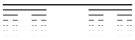
\includegraphics[width=5cm]{CantorSet}
	\centering
	\captionsetup{justification=centering}
	\caption{Cantor Set (first 6 iterations)}
	\label{fig:CantorSet}
	\vspace{-1.5cm}
\end{wrapfigure}
\paragraph{Cantor Set}
The (middle third) Cantor set $C \subseteq \left[ 0,1 \right] $ is constructed via the following informal definition:
\begin{itemize}
	\item Start with $C_0 = \left[ 0,1 \right]$
	\item Generate iteratively $C_n = \frac{C_{n-1}}{3} + \frac{2 + C_{n-1}}{3}$
	\item Take the limit $C = \lim_{n \to \infty} C_n$
\end{itemize}

The Cantor set satisfies $C = \frac{C}{3} + \frac{2 + C}{3}$, so rescaling by $\frac{1}{3}$, it contains two copies of itself.
So the intuitive Hausdorff dimension for the Cantor set is $\dim_H(C) = \frac{\log(2)}{\log(3)} \approx 0.631$.
This can be proved rigorously (see \cite[p. 34-35, ex. 2.7]{Falconer_1990}.

Another equivalent definition for the cantor set $C$ is "points in $\left[ 0,1 \right]$ with extension in base 3 composed of 0 and 2 only".
That is:
$$
C = \left\lbrace x \in \left[ 0,1 \right] \mid x = \sum_{k=1}^{\infty} x_k 3^{-k}, \ \ x_k \in \{0,2\} \ \forall k \right\rbrace
$$
From this definition, it is straightforward that the Cantor set is totally disconnected.
In fact, fractals with Hausdorff dimension smaller than 1 are totally disconnected (\cite[p. 33, prop. 2.5]{Falconer_1990}).

\begin{wrapfigure}{r}{5cm}
	\vspace{-0.5cm}
	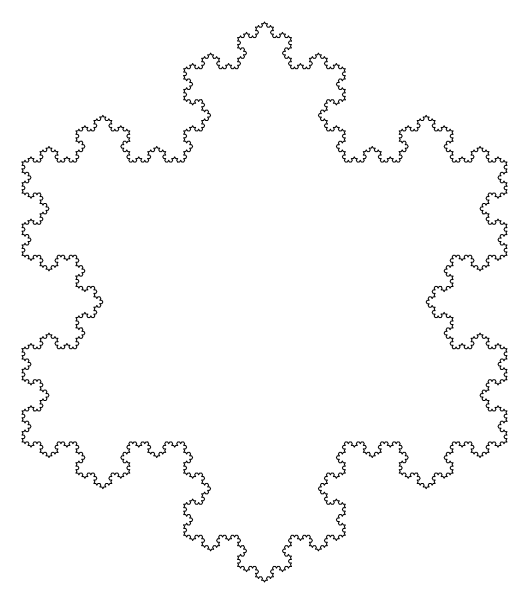
\includegraphics[width=5cm]{KochSnowflake}
	\centering
	\captionsetup{justification=centering}
	\caption{Koch Snowflake Curve Plot (5 iterations)}
	\label{fig:KochSnowflake}
\end{wrapfigure}
\paragraph{Koch Snowflake}
The Koch Snowflake is an example of a fractal curve.
Fractal curves are obtained by applying the same transformation recursively to each segment of the previous iteration of the curve.
Their fractional dimension is in the interval $\left[ 1,2 \right]$ (or in $\left[ 1,3 \right]$ if the curve evolves in a three dimensional space).

The Koch snowflake is obtained after replacing each edge of an equilateral triangle by a Koch curve with the triangle edge as initial segment.

Now, the Koch curve is defined recursively as follows:
$K_n$ is the curve at iteration $n$, with segments $K_n^1, \dots K_n^m$.
For each $i \in \llbracket 1,m \rrbracket$, split $K_n^i$ into 3 equal length segments, and replace the middle one with two new ones as on this diagram:\vspace{0.2cm}\\
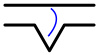
\includegraphics[width=4.5cm]{KochStep}\vspace{0.2cm}\\
Merging back all segment gives $K_{n+1}$.

The Koch curve starting form a segment $[a,b]$ is the limit curve $K = \lim_{n \to \infty} K_n$ with $K_0 = [a,b]$.

At each level, the Koch curve is scaled by $\nicefrac{1}{3}$, and $4$ copies are created.
Thus, the intuitive Hausdorff dimension for the Koch curve (which is also the dimension of the Koch snowflake) is $\dim_H(K) = \frac{\log(4)}{\log(3)} \approx 1.262$.
This can be proved rigorously using similar techniques as in \cite[p. 34-35, ex. 2.7]{Falconer_1990}.

\begin{wrapfigure}{r}{5cm}
	\vspace{-0.75cm}
	\includegraphics[width=6cm]{SierpinskiCarpet}
	\centering
	\captionsetup{justification=centering}
	\caption{Sierpinski Carpet (6 steps)}
	\label{fig:SierpinskiCarpet}
	\vspace{-5cm}
\end{wrapfigure}
\paragraph{Sierpiński Carpet}
Sierpiński carpet is a fractal constructed recursively by removing parts of its initial set.

The construction starts from a (filled) square.
Then, at each step, split every square into 9 sub-square as follows:\\
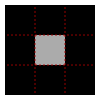
\includegraphics[width=4cm]{SierpinskiCarpetStep}\\
Remove the central square, and repeat the operation on the remaining 8 squares.

Note that this can be seen as a version of the Cantor set starting in 2 dimensions.

The figure is made of $8$ copies of itself, scaled by a factor of $\nicefrac{1}{3}$.
Therefore, the intuitive Hausdorff dimension for this set is $\dim_H(K) = \frac{\log(8)}{\log(3)} \approx 1.893$.
Again, this can be proved rigorously using similar techniques as in \cite[p. 34-35, ex. 2.7]{Falconer_1990}.


\subsubsection{Real Life Fractals}
Fractals are more than mathematical constructions, in fact self-similarity structures also occur in nature.
The limit is never reached, because of the physical constraints, but we can view them as natural approximations of fractals.
This gives a good motivation for studying fractals in a mathematical context.

\paragraph{Plants}
Some plants (not even genetically modified) have self-similarity patterns, and may therefore be considered as fractals.

\subparagraph{Ferns}
Perhaps the most obvious and popular natural fractal: Ferns leaves.
The leaves are self-similar, with varying pattern across variety of ferns.

\subparagraph{Cauliflower}
A less obvious example: Cauliflowers' surface is a fractal.
In fact, since each branch splits into about 13 branches, each about 3 times shorter, the approximate dimension of a Cauliflower's surface is $\log_3(13) \approx 2.335$.

\begin{figure}[!h]
	\centering
	\begin{subfigure}{.49\textwidth}
		\includegraphics[height=3cm]{Fern}
		\centering
		\captionsetup{justification=centering}
		\caption{Fern Leave}
		\label{fig:fern}
	\end{subfigure}
	\begin{subfigure}{.49\textwidth}
		\includegraphics[height=3cm]{Cauliflower}
		\centering
		\captionsetup{justification=centering}
		\caption{Cauliflower}
		\label{fig:cauliflower}
	\end{subfigure}
	\caption{Plant Fractals}
	\label{fig:plantsFractals}
\end{figure}

\paragraph{Coastline of Islands}
When trying to measure the length of coastlines, scientists realized that the more precise their attempt was, the higher was the value of the length found.
In fact, this makes sense: the approximation of a curve with shorter segments will capture more of the smaller curve details, resulting in a longer length.
The approximate length found could be made really large after approximating using smaller and smaller segments (until physical boundary are reached).
This yields the fact that the coastline is a fractal with dimension greater than one.

Using electronic maps, we try to estimate the fractal dimension of the coastlines for the UK islands, Iceland and Madagascar.
More details on the calculations techniques used are given in the appendix (see \ref{appendix:coastlines}).
The (approximate) coastline dimension for UK, Iceland, and Madagascar are respectively $1.24$, $1.25$, and $1.06$.

The coastlines of the UK and Iceland are much more irregular than the one of Madagascar.
The approximate values found for coastlines dimensions therefore make sense.
